
\section{State of the Art}
\subsection{General framework}
%Eficientica Energética en CPDs
%Subida de la densidad de potencia porque aumenta el número de racks aunque aumente la eficiencia energética
%PUE

There is several research on how to reduce power consumption in data centers. Those that are more relevant to this thesis are explained below. This research is focused on several lines: Reducing the consumption of the servers, improving the PUE of the data centers, rising the power density in racks and establishing new actuation techniques to manage servers. These are some of the most important works related to this topic:

\begin{itemize}
    \item As shown by Koomey in 2011 \cite{koomey2011growth}, IT sector must be concerned about data centers consumption. Despite power consumption has not raised as it was expected due to the economic crisis and to the fact that infrastructure providers have understood that they had to minimize the power consumption, the electricity used in global data centers in 2010 was between 1.1\% and 1.5\% of total electricity use. This factor is one of the reasons of this thesis.
    
\item Work by Emerson \cite{emersonDC} shows how power consumption density will increase in data centers in next years. The idea is that data centers need to incorporate new servers every week to absorb the current demand. This, supplemented by a continuous growth of the power density of the servers, makes very important to make servers more efficient.
    %http://www.emersonnetworkpower.com/en-US/Latest-Thinking/Data-Center-2025/Documents/002401_DataCenter2025Report_HR_INTERACTIVE.PDF
    %[6] de aqui? file:///C:/Users/alvaro.m.lopez/Downloads/00%20ALVARO/publications-devel/mzapater_IGSC15_submitted.pdf

    \item A key challenge is to achieve a good trade-off between energy savings and server performance. Accordingly, few researchers have recently started to investigate coordinated solutions for performance and power management in a dynamic cloud environment \cite{Kumar:2009:VLC:1555228.1555262}. The point is that the best policy for a subsystem does not depend only on the subsystem, but also the full environment. 
%http://dl.acm.org/citation.cfm?id=1555262

    \item PUE is considered one of the key metrics of the good performance and green design data centers. First, it was published by The Green Grid in 2007 as the reference metric of power usage effectiveness, due to the comparison that PUE makes between the consumption of the servers and the total consumption of the server. The most important considerations about PUE and why there are better metrics, are collected from the Green Grid in these documents \cite{amer2013pue} \cite{GreenGrid2010Eff}.
    
        %http://www.thegreengrid.org/~/media/WhitePapers/WP49-PUE%20A%20Comprehensive%20Examination%20of%20the%20Metric_v6.pdf?lang=en
        %http://www.energystar.gov/ia/partners/prod_development/downloads/Data_Center_Metrics_Task_Force_Recommendations_V2.pdf?6107-55e3
\end{itemize}


\subsection{Energy Efficiency Metrics}

%% Sería importante hablar sobre esto?
%%http://www.infoq.com/articles/power-consumption-servers

All the waste and data mentioned above are really important, but it is necessary to have some metrics to compare several DCs. The most extended metric is the Power Usage Effectiveness (PUE).

PUE is a measure defined by The Green Grid that tell us how efficient is the usage of the energy of the DC comparing the energy spent in the IT environment and all the energy spent in the DC. \cite{originalPUE}
 

\begin{equation*}
PUE = \frac{Total Facility Energy}{IT Energy}
\end{equation*}

Looking at this equation, the following keys can be extracted:

\begin{wrapfigure}{l}{0.5\textwidth}
    \centering
    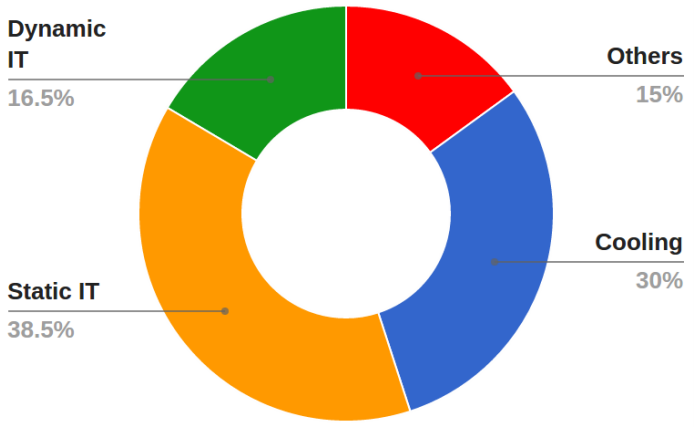
\includegraphics[width=0.5\textwidth]{percConsumoDC}
    \caption{Data center power usage distribution}

\end{wrapfigure}



Notice that PUE is always higher than 1 because IT Energy is contained in Total Facility Energy.

The perfect PUE would be 1. In this case, all the energy consumed  by the IT - servers, storage, network equipment... - would be the entirety of the energy consumption. This would be the ideal situation and there are no DC with this effectiveness.

Figure \ref{fig:pue-average} represents the evolution of PUE in Google's DCs along the last eigth years. Google DCs are considered one of the most power effective DCs around the world since they have the lowest PUE.

\begin{figure}[h]
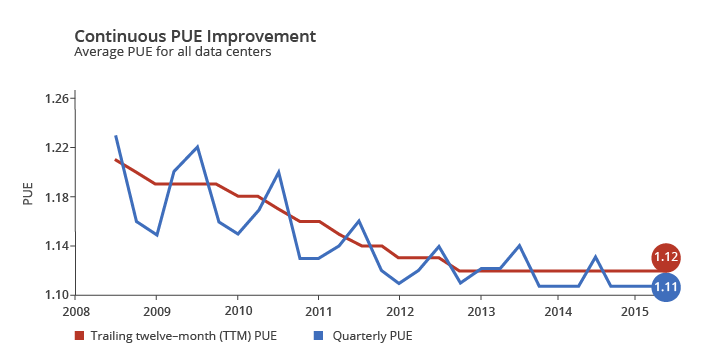
\includegraphics[scale= 0.5]{pue-average} % Podría poner[width=\linewidth]
\caption{PUE evolution of Google's DCs |\cite{puegrafica}}
\label{fig:pue-average} %Establece una etiqueta para la figura
\end{figure}
%\ref{fig:pue-average} % Devuelve el número de la figura
%\pageref{fig:pue-average} %Devuelve la página en la que está la figura

As can be seen in the plot, the PUE of Google DCS has progressively decrease year by year becoming almost 1 recently.

\subsubsection{Limitations of PUE \cite{ignacioPaper}} 

Even though, it seems a good idea to compare DCs depending on the PUE, PUE it is not the only comparison we should make talking about energy effectiveness.

As it was mentioned above, there are two contributors to the energy consumption: The server and the rest of the subsystems, and in this thesis we will focus on the consumption of the servers. According to the PUE formula, if the IT consumption is reduced, the PUE increases despite of the total energy consumption has been minimized and the DC has become more efficient.

Consequently, it can be said that PUE is a really important metric that has to be kept in mind, but it cannot be the single metric and must go with absolute metric such as consumption per server or consumption per full-load hour of each server. \cite{amer2013pue}

\subsection{Open Compute Project}

In April 2011, was announced the Open Compute Project (OCP). This project is led by Facebook with the aim of designing more efficient data centers. All the policies and designs introduced by the OCP have the same idea: making the DC a single environment where all the components - servers, building and software - can work at the same time and synchronized so that power-consumption and load share policies don't take decisions according to one component but to all the DC.

To achieve it, they share some specifications so that companies can create a new server based on the OCP specifications and, finally, the community can check if it really minimizes the energy-consumption and suggest some improvements. In this Bachelor Thesis an Intel version of the OCP server specification called Decathlete is used.

The reason why the OCP context has been chosen to work is that it is a four-years project in which some of the most important companies of the DC sector has worked. 

Finally, it is important to mention that OCP has some principles that share with this Bachelor Thesis. The most important points are the following ones:

\begin{itemize}
    \item First of all, it is based in Open Software and Hardware. Everyone can make and test its own changes without any restriction. This improves the speed at which the design upgrades.
    \item Second, OCP promotes a big research community. All new ideas are well-received at first. Then, the OCP decides which are the contributions that suit more the project and incorporates them to the main project.
    \item Thirdly, the main objective of the OCP is to create a new open standard so that several vendors could use the same standard.
\end{itemize}

\subsection{Green LSI framework}

Within this general framework, the Green LSI team also wants to participate in the optimization of the power-consumption of DC. Our work is focused on making the DC a single environment where all the components run at the same time. This synchronization is mainly targeted to reducing the power consumption. 

This thesis will be useful for the Green LSI researches for two reasons
:
\begin{itemize}
\item[$-$] Firstly, several lines of work of the GreenLSI has the aim of creating high level policies that do not have actuation support. It is a need of the group to create the tools to implement this policies in the group servers.

\item[$-$] Secondly, the results of this thesis can be applied to every server of the group so every line of work will have low-level support.
\end{itemize}
%%During this year, several works of the GreenLSI has been published.
%%Podría hablar de juan carlos y de marina como dos ejemplos del green lsi


%2015-ieee-cloudd = Marina
%2015-igsc = Marina
%2014-tpds = Zapater 
%Van los tres aquí



\subsection{Current Server-control Policies}
%Vasic N et al (2009) Making cluster applications energy-aware. In: Proc of automated ctrl for datacenters and clouds
%http://citeseerx.ist.psu.edu/viewdoc/download;jsessionid=0BAF373A528501F6B3ABF23028EBC947?doi=10.1.1.169.6157&rep=rep1&type=pdf
%46. Srikantaiah S et al (2008) Energy aware consolidation for cloud computing. In: Proc of HotPower
%http://research.microsoft.com/pubs/75408/srikantaiah_hotpower08.pdf

%Paper de alfonso
%Paper de ignacio
%Cualquier politica de actuación que solo hable de cómo manejar el consumo
As we can see in th paragraphs above, some policies at different levels inside the DC - servers, racks, hole DC - have been mentioned. One of them is at server level. Policies at server level need actuation support to implement them.

There are several research works focused on changing the configuration of a server to improve its performance, minimizing its consumption or a combination of both.

 
\begin{itemize}
    \item Research by Aransay et.al, in \cite{ignacioPaper} suggests a new algorithm to decide in which server should be allocated a new task in a data center. This algorithm recommends to use a Reputation System. Each server will have a reputation calculated using their CPU temperature and the most suitable server to allocate new workload will be established using this algorithm.

    \item In research by Felter et.al, \cite{Felter:2005:PAR:1088149.1088188}, they reduce peak power consumption by using workload-guided dynamic allocation of power among components. The idea is that not all the workloads need the same resources and these resources can be switched between power-saving and performance depending on the necessities.
    
    \item This document \cite{export:75408} suggests to consolidate applications in cloud-computing to reduce the energy consumption. This is because when an application needs low resources, the idle consumption predominate over the dynamic consumption so the server is not taking advantage of its resources. When applications are consolidated, this issue disappears.
    
    
\end{itemize}

    




